\pgfsetplotmarksize{0pt}
 \centering
 \caption{\label{tsp_conv0}brazil58},
 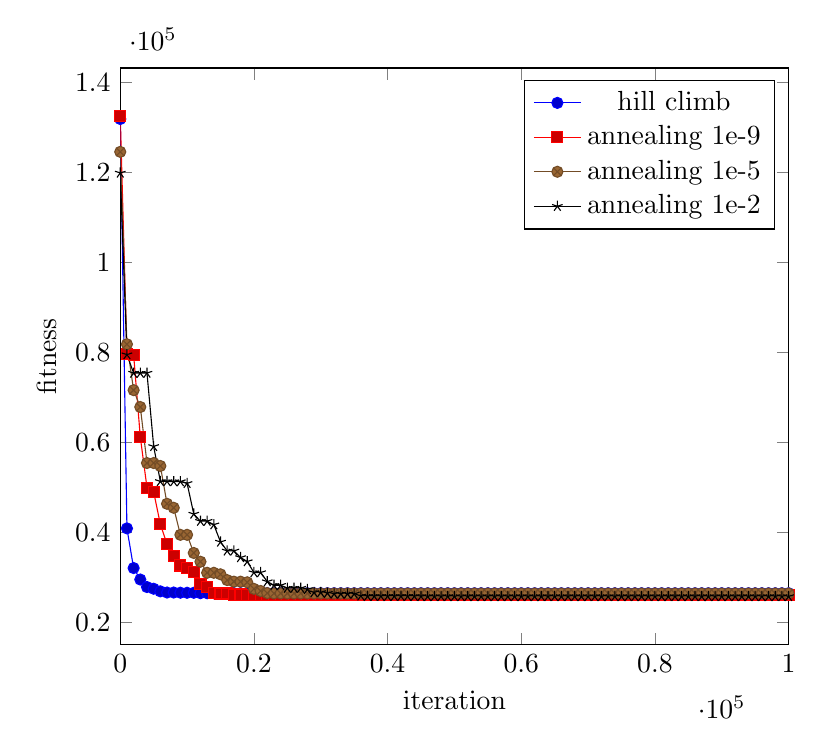
\begin{tikzpicture}
 \begin{axis}[
   width=0.7\textwidth,
   scale only axis,
   xlabel=iteration,
   ylabel=fitness,
   xmin=0,xmax=100000,
   domain=0:100000]
   \addplot coordinates {
     (0,131817)
     (1000,40879)
     (2000,32066)
     (3000,29518)
     (4000,27849)
     (5000,27470)
     (6000,26893)
     (7000,26633)
     (8000,26633)
     (9000,26590)
     (10000,26576)
     (11000,26576)
     (12000,26483)
     (13000,26483)
     (14000,26483)
     (15000,26483)
     (16000,26483)
     (17000,26483)
     (18000,26483)
     (19000,26483)
     (20000,26483)
     (21000,26483)
     (22000,26483)
     (23000,26483)
     (24000,26483)
     (25000,26483)
     (26000,26483)
     (27000,26483)
     (28000,26483)
     (29000,26483)
     (30000,26483)
     (31000,26483)
     (32000,26483)
     (33000,26483)
     (34000,26483)
     (35000,26483)
     (36000,26483)
     (37000,26483)
     (38000,26483)
     (39000,26483)
     (40000,26483)
     (41000,26483)
     (42000,26483)
     (43000,26483)
     (44000,26483)
     (45000,26483)
     (46000,26483)
     (47000,26483)
     (48000,26483)
     (49000,26483)
     (50000,26483)
     (51000,26483)
     (52000,26483)
     (53000,26483)
     (54000,26483)
     (55000,26483)
     (56000,26483)
     (57000,26483)
     (58000,26483)
     (59000,26483)
     (60000,26483)
     (61000,26483)
     (62000,26483)
     (63000,26483)
     (64000,26483)
     (65000,26483)
     (66000,26483)
     (67000,26483)
     (68000,26483)
     (69000,26483)
     (70000,26483)
     (71000,26483)
     (72000,26483)
     (73000,26483)
     (74000,26483)
     (75000,26483)
     (76000,26483)
     (77000,26483)
     (78000,26483)
     (79000,26483)
     (80000,26483)
     (81000,26483)
     (82000,26483)
     (83000,26483)
     (84000,26483)
     (85000,26483)
     (86000,26483)
     (87000,26483)
     (88000,26483)
     (89000,26483)
     (90000,26483)
     (91000,26483)
     (92000,26483)
     (93000,26483)
     (94000,26483)
     (95000,26483)
     (96000,26483)
     (97000,26483)
     (98000,26483)
     (99000,26483)
     (100000,26483)
   };
   \addlegendentry{hill climb}
   \addplot coordinates {
     (0,132467)
     (1000,79683)
     (2000,79453)
     (3000,61156)
     (4000,49924)
     (5000,48964)
     (6000,41805)
     (7000,37400)
     (8000,34659)
     (9000,32648)
     (10000,31995)
     (11000,31200)
     (12000,28565)
     (13000,27839)
     (14000,26586)
     (15000,26414)
     (16000,26414)
     (17000,26183)
     (18000,26175)
     (19000,26140)
     (20000,26133)
     (21000,26133)
     (22000,26133)
     (23000,26133)
     (24000,26133)
     (25000,26112)
     (26000,26112)
     (27000,26112)
     (28000,26112)
     (29000,26112)
     (30000,26112)
     (31000,26112)
     (32000,26112)
     (33000,26112)
     (34000,26112)
     (35000,26112)
     (36000,26112)
     (37000,26112)
     (38000,26112)
     (39000,26112)
     (40000,26112)
     (41000,26112)
     (42000,26112)
     (43000,26112)
     (44000,26112)
     (45000,26112)
     (46000,26112)
     (47000,26112)
     (48000,26112)
     (49000,26112)
     (50000,26112)
     (51000,26112)
     (52000,26112)
     (53000,26112)
     (54000,26112)
     (55000,26112)
     (56000,26112)
     (57000,26112)
     (58000,26112)
     (59000,26112)
     (60000,26112)
     (61000,26112)
     (62000,26112)
     (63000,26112)
     (64000,26112)
     (65000,26112)
     (66000,26112)
     (67000,26112)
     (68000,26112)
     (69000,26112)
     (70000,26112)
     (71000,26112)
     (72000,26112)
     (73000,26112)
     (74000,26112)
     (75000,26112)
     (76000,26112)
     (77000,26112)
     (78000,26112)
     (79000,26112)
     (80000,26112)
     (81000,26112)
     (82000,26112)
     (83000,26112)
     (84000,26112)
     (85000,26112)
     (86000,26112)
     (87000,26112)
     (88000,26112)
     (89000,26112)
     (90000,26112)
     (91000,26112)
     (92000,26112)
     (93000,26112)
     (94000,26112)
     (95000,26112)
     (96000,26112)
     (97000,26112)
     (98000,26112)
     (99000,26112)
     (100000,26112)
   };
   \addlegendentry{annealing 1e-9}
   \addplot coordinates {
     (0,124519)
     (1000,81784)
     (2000,71585)
     (3000,67836)
     (4000,55397)
     (5000,55397)
     (6000,54743)
     (7000,46341)
     (8000,45454)
     (9000,39448)
     (10000,39448)
     (11000,35419)
     (12000,33478)
     (13000,31016)
     (14000,31016)
     (15000,30678)
     (16000,29392)
     (17000,29048)
     (18000,29048)
     (19000,28905)
     (20000,27444)
     (21000,26973)
     (22000,26508)
     (23000,26450)
     (24000,26445)
     (25000,26433)
     (26000,26433)
     (27000,26433)
     (28000,26433)
     (29000,26433)
     (30000,26433)
     (31000,26433)
     (32000,26433)
     (33000,26433)
     (34000,26428)
     (35000,26428)
     (36000,26428)
     (37000,26428)
     (38000,26428)
     (39000,26428)
     (40000,26428)
     (41000,26428)
     (42000,26428)
     (43000,26428)
     (44000,26428)
     (45000,26428)
     (46000,26428)
     (47000,26428)
     (48000,26428)
     (49000,26428)
     (50000,26428)
     (51000,26428)
     (52000,26428)
     (53000,26428)
     (54000,26428)
     (55000,26428)
     (56000,26428)
     (57000,26428)
     (58000,26428)
     (59000,26428)
     (60000,26428)
     (61000,26428)
     (62000,26428)
     (63000,26428)
     (64000,26428)
     (65000,26428)
     (66000,26428)
     (67000,26428)
     (68000,26428)
     (69000,26428)
     (70000,26428)
     (71000,26428)
     (72000,26428)
     (73000,26428)
     (74000,26428)
     (75000,26428)
     (76000,26428)
     (77000,26428)
     (78000,26428)
     (79000,26428)
     (80000,26428)
     (81000,26428)
     (82000,26428)
     (83000,26428)
     (84000,26428)
     (85000,26428)
     (86000,26428)
     (87000,26428)
     (88000,26428)
     (89000,26428)
     (90000,26428)
     (91000,26428)
     (92000,26428)
     (93000,26428)
     (94000,26428)
     (95000,26428)
     (96000,26428)
     (97000,26428)
     (98000,26428)
     (99000,26428)
     (100000,26428)
   };
   \addlegendentry{annealing 1e-5}
   \addplot coordinates {
     (0,119830)
     (1000,79479)
     (2000,75385)
     (3000,75385)
     (4000,75385)
     (5000,59093)
     (6000,51315)
     (7000,51315)
     (8000,51281)
     (9000,51281)
     (10000,50895)
     (11000,44069)
     (12000,42484)
     (13000,42484)
     (14000,41698)
     (15000,37860)
     (16000,35884)
     (17000,35884)
     (18000,34417)
     (19000,33511)
     (20000,31073)
     (21000,31073)
     (22000,29056)
     (23000,28250)
     (24000,28250)
     (25000,27619)
     (26000,27619)
     (27000,27619)
     (28000,27336)
     (29000,26655)
     (30000,26655)
     (31000,26494)
     (32000,26319)
     (33000,26319)
     (34000,26319)
     (35000,26318)
     (36000,25886)
     (37000,25808)
     (38000,25808)
     (39000,25808)
     (40000,25808)
     (41000,25808)
     (42000,25808)
     (43000,25808)
     (44000,25808)
     (45000,25774)
     (46000,25766)
     (47000,25766)
     (48000,25766)
     (49000,25766)
     (50000,25761)
     (51000,25761)
     (52000,25761)
     (53000,25761)
     (54000,25761)
     (55000,25761)
     (56000,25761)
     (57000,25761)
     (58000,25761)
     (59000,25761)
     (60000,25761)
     (61000,25761)
     (62000,25761)
     (63000,25761)
     (64000,25761)
     (65000,25761)
     (66000,25761)
     (67000,25761)
     (68000,25761)
     (69000,25761)
     (70000,25761)
     (71000,25761)
     (72000,25761)
     (73000,25761)
     (74000,25761)
     (75000,25761)
     (76000,25761)
     (77000,25761)
     (78000,25761)
     (79000,25761)
     (80000,25761)
     (81000,25761)
     (82000,25761)
     (83000,25761)
     (84000,25761)
     (85000,25761)
     (86000,25761)
     (87000,25761)
     (88000,25761)
     (89000,25761)
     (90000,25761)
     (91000,25761)
     (92000,25761)
     (93000,25761)
     (94000,25761)
     (95000,25761)
     (96000,25761)
     (97000,25761)
     (98000,25761)
     (99000,25761)
     (100000,25761)
   };
   \addlegendentry{annealing 1e-2}
 \end{axis}
 \end{tikzpicture}
